\subsection*{b)}

Here we construct our hybrid MCMC algorithm to sample from the posterior $f(\theta,\boldsymbol{\lambda},\boldsymbol{t}|\boldsymbol{\tau})$. All components except the breakpoints $\boldsymbol{t}$ have been updated using Gibbs sampling, which is explained in further down in this section. The Metropolis--Hastings algorithm is explained below and has been used for the posterior of $\boldsymbol{t}$. Where we, as already mentioned, used a symmetric proposal for the proposal kernel. We will now briefly discuss the two different algorithms used for sampling.
\begin{itemize}
\item{The \textbf{Metropolis--Hastings} algorithm is an algorithm that is used for sampling from high--dimensional and/or complicated distributions that are for example only known up to a normalizing constant. The idea behind the MH algorithm is to choose a transition density $q$ almost arbitrarily. However, this density will not give the desired asymptotic distribution $f$, i.e. the distribution from which you wish to sample. We correct this by introducing a new transition density $\hat{q}$ using $q$ and a probability $\alpha(x,x^*)$ where $x$ is the current level and $x^*$ is a proposal. The proposal $x^*$ is rejected with probability $1 - \alpha(x,x^*)$. In order for the global balance equation to be satisfied, we must have that $\alpha(\cdot,\cdot)$ is defined as 
\[\alpha(x,x^*) = \min \left ( 1, \frac{f(x^*)q(x|x^*)}{f(x)q(x^*|x )} \right ) .\]
Since we now have a quotient, we can easily sample from distributions known only up to normalizing constants.
In our case we have, as already mentioned, a symmetric proposal. Which practically means that $q(x^*|x ) = q(x|x^* )$ and the two right terms of the quotient cancel out. The MH algorithm is explained briefly in figure \ref{fig:metrohast}.
\begin{figure}[H]
  \centering
    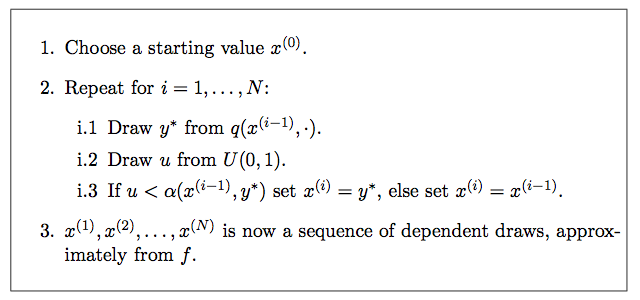
\includegraphics[scale=0.34]{./Figures/metrohast.png}
  \caption[An Electron]{Overview of how the Metropolis--Hastings algorithm works. The figure is taken from the lecture notes by Martin Sk\"old.}
  \label{fig:metrohast}
\end{figure}
}

\item{The \textbf{Gibbs sampler} algorithm is a Markov Chain Monte Carlo (MCMC) algorithm for obtaining a sequence of observations, which in turn can be approximated from a multivariate probability distribution. Typically the Gibbs sampler is used to approximate joint distributions, marginal distributions of one variable or computing an integral, when some of the variables are known observations, and is not in need of sampling. As this a MCMC algorithm, Gibbs sampling generates a Markov Chain of samples, hence the beginning of the chain may not accurately describe the desired distribution and one may want to remove the burn-in of the chain. Below a brief description of the algorithm is presented

\begin{enumerate}
	\item{Assuming we want to sample from multivariate distribution f on X. Assuming that X can be divided into blocks.}
	\item{We denote $x^k$ by the \textit{k}th component and $x^{-k}$ by the remaining components. Assuming that it is easy to simulate from $f_k(x^k|x^{-k}),\forall k$, i.e. the conditional distribution of $X^k$ given the other components.}
	\item{Now, simulating a sequence $X_k$, forming a Markov Chain on X, with the following properties: Given $X_k$, draw $X_{k+1}^n \sim f_n(x^n|x^{-n})$.}
\end{enumerate}
}
\end{itemize}


%\textit{Random walk proposal:} update one breakpoint at a time. For each breakpoint $t_i$ we generate a candidate $t_i^*$ according to

%\begin{equation*}
%t_i^*=t_i+\epsilon, \quad \text{with} \quad \epsilon \sim U(-R,R), \quad R=\rho(t_{i+1}-t_{i-1}
%\end{equation*}
The symmetric proposal yields a correct MCMC algorithm, as long as the proposal kernel specifies an irreducible aperiodic Markov Chain. The algorithm will generate a reversible Markov Chain with stationary distribution $\pi$, assuming that $\chi$ is a subset of $\mathbb{R}^k$ and the transition kernel $r(z|x)$ and $\pi(z)$ are densities on $\chi$. \\

The proposed kernel yields a correct MCMC as we have introduced a symmetric proposal, thus
\begin{equation}
r(z|x)=r(x|z), \quad \forall (x,z) \in t
\end{equation}
%http://dept.stat.lsa.umich.edu/~yvesa/afmp.pdf
implying that we can reach each state from any state and is non-periodic, i.e. an irreducible aperiodic Markov Chain.
